\chapter{CT RECONSTRUCTION}
\label{chap:reconstruction}

The essential goal any reconstruction is to use the information gathered to find out what the object looks like.  In the case of CT, we use the information gathered on the detector over a range of angles to reconstruct the x-ray attenuation coefficient of the object.  CT system as evolved tremendously over the years and reconstruction algorithm has also evolved dramatically to support the types of systems. Over the years, reconstruction techniques has evolved using two general approaches to reconstruction, analytical and iterative method.  In this chapter we attempt to give a brief overview of these general techniques used for CT reconstruction in the first section, then we will explain the method that was used for our system.

The first clinical CT scanner was installed in 1971 where it used a single detector and was only dedicated to brain imaging only.  Soon after, a whole body CT scanner was introduced in 1973~\citep{Ulzheimer2009}.  Up until 1990, most clinical CT scanners used the fan-beam geometry with axial rotation.  In the early 1990s, out of the desire to cover an entire human organ, the first single-slice helical/spiral CT was introduced.  Ever since then, the spiral geometry became the main configuration for all clinical CT scanners.  Eliscint was the first to develop a two-slice CT system in the mid 1990's.  A few years later, GE came out with the first four-slice CT scanner and was quickly followed by all other major CT manufacturers.  The term multislice CT also called multi-detector row CT (MDCT) quickly became the trend with manufacturers pushing for more, from 16 slices in 2002~\citep{Impact2002} to 320 slices in the late 2007 by both Philips and Toashiba~\citep{Ulzheimer2009}.  While industry has been pushing for larger volume coverage and faster scan time, it fueled the need to develop newer, and more efficient reconstruction algorithms.

\subsection{Analytic Reconstruction Techniques}

The most common method of image reconstruction for the earlier CT scanners were the fan-beam axial filtered back-projection algorithm.  At the heart of the reconstruction algorithm is the Radon transform, which relates a function $f(\mathbf{r})$ to the collection of line integrals of that function $\lambda(p, \phi)$.  Shown in Eq.~\ref{eq:radon}, the equation of the projection line is $\mathbf{r \cdot \hat{n}} = p$, where $\mathbf{\hat{n}}$ is a unit vector making an angle $\phi$ to the x-axis, show on Fig.~\ref{fig:RadonTransform}.  

\begin{equation}
\lambda(p, \phi) = \int_\infty d^2r \; f(\mathbf{r}) \delta(p- \mathbf{r} \cdot \mathbf{\hat{n}}).
\label{eq:radon}
\end{equation}

\begin{figure}[h]
\centering

\includegraphics[scale=1]{Radon_transform.eps}
\caption{2D Radon transfrom }
\label{fig:RadonTransform}
\end{figure}

\noindent To solve the Radon transform, the projection data on the detector at each angle goes through a Fourier transform, which mathematically represents the object data in frequency space along the projection angle.  The Fourier transformed data is then filtered in the spatial frequency by a ramp filter then back-projected into object space to reconstruct the original object.  This is also known as the Filtered back-projection (FBP) technique.  To solve for the fan-beam geometry, typically the projection data are gathered and rebinned into parallel sets before taking the inverse Radon transform to obtain the reconstructed slices.

CT scanning geometry can be divided into two general categories depending on the targeted region of interest (ROI) within the body.  First is circular/axial orbit scanning.  This is usually used to image smaller features of the body such as coronary artery, brain or the heart.  The circular scanning geometry has the advantage of being very simple and fast, especially when the data acquired needs to be synchronized with a physiological signal, such as an EKG.  The most widely used reconstruction algorithm is the Feldkamp-Davis-Kress (FDK) reconstruction (Feldkamp2008).  The algorithm is very similar to the conventional fan-beam reconstruction where the off-axis rays of the cone beam are weighted by a cosine term in order to approximate them as the 2D fan-beam rays.  The FDK algorithm works well when cone angle is moderate, and many authors have proposed alternative methods to fix and compensate the image slices at the outer edges of the cone beam~\citep{Katsevich2003, Chen2003, Hu1996}.

The second type and the most widely used scanning method is the helical/spiral geometry.  Approach to solve the helical cone beam reconstruction can be generally divided into two categories: approximate and exact reconstruction methods.  The most common method to solving this problem is the approximate reconstruction technique derived from the original FDK algorithm and later generalized to spiral scan first by Ge Wang~\citep{Wang1993}.  Many authors have also succeeded in creating helical cone-beam algorithms based on the Feldkamp method~\citep{Wang1992, Kudo1991, Yan1992, Smith1992, Noo1999, Kachelriess2000, Tang2004, Tang2006a, Tang2006b}.  As noted by Wang, \textit{The key idea is to correct cone-beam data into fan-beam counterpants in a heuristic way.  As a primary example, a cone-beam datum along an oblique ray can be approximately converted to the fan-beam counterpart along a transverse ray by multiplying the former with the cosine of the angle between the oblique and transverse rays}~\citep{Wang2007}.

\begin{figure}[h]
\includegraphics[width = 13cm]{Tam_figure.PNG}
\caption{Spiral-and-two-circles scan path for ROI imaging as proposed by Tam et al~\citep{Tam1998}.}
\label{fig:tam_circle}
\end{figure}

Methods of solving for exact cone beam image reconstruction have been independently reported by Tuy, Smith, and Grangeat as early as 1983~\citep{Tuy1983, Smith1985, Grangeat1991}.  The requirements in all of these algorithms is that the object must be completely covered by the detector from all view angles.  However, objects in medicine and many industrial inspections are very long, which will require a very large area detector to cover the entire length of the object.  Not to mention, in most of these objects, only a smaller section is of interest.  The problem of solving for a smaller ROI without scanning the entire object is extremely challenging.  Intuitively, we need to collect all the x-ray paths that penetrates the ROI for reconstruction.  However parts of these x-ray beams are ``corrupted'' by other parts of the objects, so they no longer represent the ROI exclusively.  We can try to solve the ``corrupted'' parts of the x-ray paths but they are often missing because the detector was not large enough to collect all the information.  This problem is known as data truncation, or missing data.  Method of solving the exact solution to a long object problem with a ROI was proposed by Tam in 1998 using a spiral-and-two-sircle scan path for ROI imaging~\citep{Tam1998}, shown in Fig.~\ref{fig:tam_circle}.  Unfortunately it is not entire trivial to merge the truncated data from multiple helical turns,  which would also increase radiation dose and scan time.  This problem was not solved until early 2002 by Katsevich's breakthrough~\citep{Katsevich2002SIAM, Katsevich2003, Katsevich2004}.
%
%\begin{figure}[h]
%	\begin{subfigure}[b]{0.2\linewidth}
%		\includegraphics[scale=0.7]{circle-plus-line.eps}
%		\caption{}
%		\label{fig:circle-line}
%	\end{subfigure}
%	\begin{subfigure}[b]{0.2\linewidth}
%		\includegraphics[scale=0.7]{circle-plus-arc.eps}
%		\caption{}
%		\label{fig:circle-arc}
%	\end{subfigure}
%	\begin{subfigure}[b]{0.2\linewidth}
%		\includegraphics[scale=0.7]{dual-circle.eps}
%		\caption{}
%		\label{fig:dual-circle}
%	\end{subfigure}
%	\begin{subfigure}[b]{0.2\linewidth}
%		\includegraphics[scale=0.7]{saddle.eps}
%		\caption{}
%		\label{fig:saddle}
%	\end{subfigure}
%\caption{Different scanning trajectories for complete sampling. \ref{fig:circle-line}: circle-plus-line, \ref{fig:circle-arc}: circle-plus-arc, %\ref{fig:dual-circle}: dual circle, and \ref{fig:saddle}: saddle}
%\label{fig:scanning_trajectories}
%\end{figure}

\begin{figure}[h]
\includegraphics[scale=1]{scanning_trajectories}
\caption{Different scanning trajectories for complete sampling. (a) circle-plus-line (b) circle-plus-arc (c) dual circles (d) saddle}
\label{fig:scanning_trajectories}
\end{figure}

Since Katsevich's invention, various sophisticated formulas have been proposed and developed for exact reconstruction using longitudinally and transversely truncated projection data, and for various scanning geometries shown in Fig.~\ref{fig:scanning_trajectories}.  However, although these algorithms are highly sophisticated and novel, they are computationally expensive compared to the popular FBP algorithms not mention difficult to build in hardware.  Currently, most CT manufacturers still use the approximate cone-beam reconstruction algorithms instead of exact cone-beam reconstruction algorithms for two reasons.  First, the data requirements for exact reconstruction are still too difficult due to physical constraints.  Secondly, often times the approximate algorithms already provide very good sometimes even better performance compared to the exact reconstruction method, which may not have the best noise characteristics~\citep{Wang2008}.  It will be interesting to see when exact algorithm will over take approximate algorithm in the future.

\subsection{Iterative Reconstruction Techniques}
Iterative reconstruction techniques try to solve for the object using projection images in an iterative fashion, where the solution to the object at the current iteration will be used for the next iteration.  All iterative reconstruction methods consist of three major steps which are repeated iteratively until a final solution is reached.  First, a forward projection of the object creates an estimate of the raw data.  Second, the estimated raw data and the real measured data are compared and a correction term is calculated.  Third, the correction term is back projected onto the object to create a new estimate of the object.  Shown in Fig.~\ref{fig:generalIR}, this process is repeated until either a fixed umber of iteration is reached or the object estimation reaches a predefined criterion.

\begin{figure}
\centering
\includegraphics[width = 13cm]{iterative_recon_process.png}
\caption{The general process of iterative algorithm~\citep{Beister2012}.}
\label{fig:generalIR}
\end{figure}

\subsection{Algebraic Iterative reconstruction techniques}
From a historical perspective, the very first reconstructed CT image was created using the algebraic iterative reconstruction (ART) method where the method tries find the object by solving a series of linear equations, $\mathrm{A\,\mathbf{x} = \mathbf{b}}$.  In terms of image reconstruction $\mathrm{\mathbf{x}}$ are the object voxels that need to be reconstructed, $\mathrm{A}$ is the system matrix used for producing the raw data and $\mathrm{\mathbf{b}}$ are the pixels of the measured raw data.  The entries of the matrix $\mathrm{A}$ correspond to x-rays from the source through the object volume to the detector pixels.  Solving for the object voxels involves inverting the large matrix A.  Starting from ART, there evolved a series of algorithms that would try to converge to the solution faster, reduce noise, reduce problems with streak artifacts, but in general all ART-based methods are non-statistical and model the geometry of the acquisition process better than common analytical methods based on FBP.  Therefore ART-based methods can better deal with sparse data and an irregular sampling of acquisition positions\citep{Beister2012}.

\subsection{Statistical Iterative reconstruction techniques}
Statistical iterative reconstruction techniques has been used extensively in single photon emission tomography (SPECT) and positron emission tomography (PET) where low photon rates and noise are major issues.  Since the increase in public awareness of CT radiation and a need to reduce the risks associated with radiation, transitioning to statistical iterative reconstruction techniques has the potential of lowering radiation dose while suppressing image noise from low-dose scan techniques.  Therefore, it is crucial that the mathematical model of the CT image system is accurate for the success of the reconstruction algorithm to ensure modeling errors are suppressed and does not grow and form artifacts in the iterative process.  There are two types of models that are typically use in the iterative reconstruction algorithm, a physical model that involves the geometry of the system and a statistical model that tries to formulate the noise within the imaging system.

Unlike analytical reconstruction where numerous physical assumptions were used to make the mathematics manageable.  For example, the size of the x-ray focal spot is assumed to be infinitely small, the shape and dimension of each detector cell are ignored, and all x-ray photon interactions are assumed to take place at a point located at the geometric center of the detector cell.  Iterative reconstruction requires no prior assumptions about the geometry of the system.  Iterative reconstruction allows for better modeling of the image forming process and can account for any physical process limited by the computational power of the current computer.  For example, a commonly used model is to cast multiple pencil rays through the x-ray focal spot, image voxel, and the detector pixel to mimic different x-ray photon paths going through the object and the summation of the rays on each detector are used to approximate the CT image forming system. Needless to say, this method is extremely time consuming.  Another commonly used approach is to model the "shadow" cast by each image voxel onto the detector and rely on the point-response function to model the forward projection process of the CT system, where the response function is non-stationary and changes with the voxel location to account for different magnifications and orientations.  Comparatively, this method is computationally more efficient.  Shown in Fig~\ref{fig:physical_modeling}.



\begin{figure}

	\begin{subfigure}[b]{0.4\linewidth}

	\includegraphics[width = 7cm]{pencil_beam_model.png}	
	\end{subfigure}
\hspace{0.2cm}
	\begin{subfigure}[b]{0.4\linewidth}

	\includegraphics[width = 7cm]{psf_model.png}
	\end{subfigure}
\caption{examples of physical modeling in Hsieh's paper}
\label{fig:physical_modeling}
\end{figure}

The statistical model or the noise model tries to incorporate the statistics of the detected photon into the reconstruction process.  This may include incident photon flux variations (known as the Poisson distribution, though it is approximate due to the poly-energetic x-ray source used in CT), energy-dependent light production in the scintillator, shot noise in photo-diodes, electronic noise in readout electronics. The most common noise model is the zero-mean Gaussian noise.

Once both the geometry and the noise of CT system are properly modeled, a cost function is need to be chosen.  The iterative process is used to search for the minimum of the cost function and the solution that minimizes the cost function is the reconstructed object.  This cost function, sometimes called an objective functional, typically consist of two components, a data agreement part tries to see the difference between the experimental data and the object that generated the data based on the model, and a regularizing term sometimes called a penalty function that depends only on the object and serves as a prior such as positivity.  If the functional is strictly convex, then the minimum is unique and all algorithms should obtain the same image if run to convergence.  The only issues are then which algorithm will find the minimum most efficiently and with the least computing resources.  In practice, however, iterative algorithms may not be run to convergence, and the resulting image depends on the algorithm, the initial estimate and the stopping rule.

\section{Maximum Likelihood Expectation Maximization (MLEM) }
In this project, we used the Maximum Likelihood Expectation Maximization algorithm for the reconstruction process without any regularization functions.  The MLEM algorithm is shown in equation \ref{eq:MLEM} \citep{EmissionTom2004}, where $g$ is the projection image data vector, $H$ is the imaging matrix that relates the object voxels to image pixels, and $f$ is the object vector.  Note that this equation assumes that the detector pixels are identical and independently distributed, and each detector pixel follows a Gaussian noise model. 
\begin{equation}
\hat{f}^{(n+1)}_{j} = \frac{\hat{f}^{(n)}_j}{{\sum\limits_{i'}} h_{i'j}} \; 
						\sum\limits_{i} h_{ij} \, \frac{g_{i}}{\sum\limits_{k} h_{ik} \hat{f}_{k}^{(n)}}
\label{eq:MLEM}
\end{equation}

$\sum\limits_k h_{ik} \hat{f}_k^{(n)}$ takes the current object volume $\hat{f}^{(n)}$ and calculates its forward projection image at all angles.  These forward projected images are divided into the data image vector, $g_i$ for every angle.  The result is a ratio between a set of simulated projection images and experimental value.  This ratio is then used by the imaging matrix $\sum\limits_i \; h_{ij}$ to project back into object space.  The next iteration for object voxels is calculated by multiplying the back projected ratio by the current object volume $\hat{f}_j^{(n)}$ and divide by a sensitivity function $\sum\limits_{i'} h_{i'j}$.
The most important function in the MLEM algorithm is the imaging matrix $H$ that models the imaging system.  Commonly the $H$ matrix is a measured in the case of PET or SPECT where a point source is scanned in the entire volume of the object and the signal is recorded for every point object point at every detector pixel over all scanning angles.  This is impossible for CT because for one, the $H$ matrix would've been astronomically large and impossible to store and use, so we have opted to model the CT system to compute the forward projection and backward projection process on-the-fly instead of using a stored $H$ matrix.  This way we can re-write the MLEM equation in \ref{eq:MLEM} to a simpler equation shown in \ref{eq:MLEM_operator}.
\begin{equation}
\hat{f}^{(n+1)} = \frac{\hat{f}^{(n)}}{S} \; H^{t} \; \frac{g}{H \hat{f}^{(n)}}
\label{eq:MLEM_operator}
\end{equation}
Here, $H$ is the forward operator that takes an input object $\hat{f^{(n)}}$ into image space, where it is divided into g.  $H^t$ is the backward projector that takes all projection image ratios and back project them into object space.  This is then multiplied by a ratio of the current object and a sensitivity volume.  In the next section we will explain the CT system model and how the forward and backward projectors were calculated.
\comment{
this last bit where a ``simplier'' MLEM equation is given might not be important
}

\section{CT model and projector calculation}
The pencil beam model was used for both the forward and backward projection, where we assumed that each x-ray beam is launched from an infinitely small x-ray point source. This pencil beam travels towards the geometrical center of each detector pixel.  Along the way, the contributions from each voxel for each ray is calculated according to Siddon's algorithm \cite{Siddon1985}.  This model does not account for any scatter in the x-ray, it also assumes that the x-ray beam is monochromatic.

In the forward projector, the final value at the each of the detector element represents the summation of the product between the length of the ray that passed through each voxel and the value at each voxel.  In the backward projector, the order is reversed. We take the value at the detector element trace a ray backward through the object volume to the x-ray source.  For every voxel pierced by that ray, we calculate the length of the ray passed through the voxel and multiply it by the detector element.  This was repeated for all x-rays, i.e. all detector values.  Figure \ref{fig:forward_backward_model} demonstrates how the forward and backward projection works.

\begin{figure}
\centering
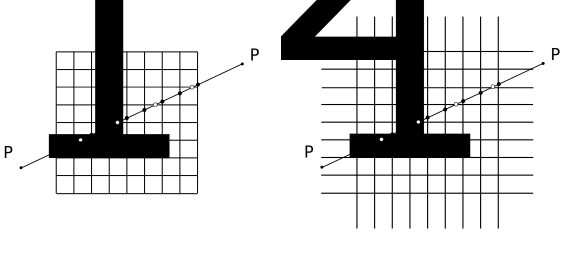
\includegraphics[scale=0.8]{siddon_proj_planes.eps}
\caption{How the forward and backward model works}
\label{fig:forward_backward_model}
\end{figure}

In the next section we will explain briefly how the Siddon's algorithm works and how we modified the algorithm so it can be implemented in CUDA. 

\subsection{Siddon's algorithm}
The Siddon's algorithm is a method of calculating the exact radiological path for a three-dimensional CT array.  Instead of directly calculating the intersections of the ray with each pixel, it calculates the ray's intersection with the three parallel planes in the object volume $\{ x, y, z \}$.  The intersection of the ray with equally spaced, parallel lines is a very simple problem.  Since the lines are equally spaced, it is only necessary to determine the first intersection.  The other intersections can then be automatically generated by recursion.  For a CT volume array of $(N_x -1, N_y-1, N_z-1)$ voxels, the orthogonal sets of equally spaced, parallel planes are written as

\begin{equation}
	\begin{aligned}
		X_{plane}(i) & = X_{plane}(1) + (i-1)\, d_x 	&(i = 1, ..., N_x),\\ 
		Y_{plane}(j) & = Y_{plane}(1) + (j-1)\, d_y  	&(j = 1, ..., N_y),\\
		Z_{plane}(j) & = Z_{plane}(1) + (k-1)\, d_z		&(k = 1, ..., N_z),
	\end{aligned}
	\label{eq:siddon_planes}
\end{equation}
where $d_x$, $d_y$, and $d_z$ are the distances between the $x$, $y$, and $z$ planes, respectively.  They are also the lengths of the sides of the voxel.  We can calculate the initial and final intersection plane of the ray with the object volume by the plane indexes by first calculating a set of minimum and maximum parametric values for each ray by the following equation

\begin{equation}
\begin{aligned}
\alpha_x(1) &= \frac{X_{plane}(1) - X_1}{X_2 - X_1} \qquad &\alpha_x(N_x) &= \frac{X_{plane}(N_x) - X_1}{X_2 - X_1}, \\
\alpha_y(1) &= \frac{Y_{plane}(1) - Y_1}{Y_2 - Y_1} \qquad &\alpha_y(N_y) &= \frac{Y_{plane}(N_y) - Y_1}{Y_2 - Y_1}, \\
\alpha_z(1) &= \frac{Z_{plane}(1) - Z_1}{Z_2 - Z_1} \qquad &\alpha_z(N_z) &= \frac{Z_{plane}(N_z) - Z_1}{Z_2 - Z_1}. \\
\end{aligned}
\label{eq:siddon_alpha_extremes}
\end{equation}

If the denominator $(X_2 - X_1)$, $(Y_2-Y_1)$, or $(Z_2 - Z_1)$ is equal to zero, then the ray is parallel to that plane, and the corresponding $\alpha_x$, $\alpha_y$, or $\alpha_z$ will be undefined and excluded from the calculation.  Once the values from equation \ref{eq:siddon_alpha_extremes} is calculated, two parametric value that can be used to indicate the initial and final intersection of the ray with the object volume is given by 

\begin{equation}
\begin{aligned}
\alpha_{min} &= max\{0, min \left[ \alpha_x(1), \alpha_x(N_x) \right], min \left[ \alpha_y(1), \alpha_y(N_y) \right], min \left[ \alpha_z(1), \alpha)z (N_z) \right], \\
\alpha_{max} &= min\{1, max \left[ \alpha_x(1), \alpha_x(N_x) \right], max \left[ \alpha_y(1), \alpha_y(N_y) \right], max \left[ \alpha_z(1), \alpha)z (N_z) \right].
\end{aligned}
\label{eq:siddon_alpha_min_max}
\end{equation}
If $\alpha_{max}$ is less than or equal to $\alpha_{min}$, then the ray does not intersect the object volume and that ray will be excluded from the calculation.  We can then calculate the indexes of the plane that will be intersected by the ray using the following equation:
\begin{equation}
	\begin{aligned}
	\text{if ($X_2 - X_1 \geq 0 )$ }\\
	i_{min} &= N_x - \left[ X_{plane}(N_x) - \alpha_{min} (X_2 - X_1) - X_1 \right] /  d_x, \\
	i_{max} &= 1 + \left[ X_1 + \alpha_{max} (X_2 - X_1) - X_{plane}(1) \right] / d_x, \\
	\text{if ($X_2 - X_1 \leq 0 )$ }\\
	i_{min} &= N_x - \left[ X_{plane}(N_x) - \alpha_{max} (X_2 - X_1) - X_1 \right] /  d_x, \\
	i_{max} &= 1 + \left[ X_1 + \alpha_{min} (X_2 - X_1) - X_{plane}(1) \right] / d_x
	\end{aligned}
\label{eq:siddon_ijkminmax}
\end{equation}
with similar expressions for $j_{min}$, $j_{max}$, $k_{min}$,and $k_{max}$.  The corresponding parametric values to each indexes can be calculated by:

\begin{equation}
\begin{aligned}
\alpha_x(i) &= \left[ X_{plane}(i) - X_1 \right] / (X_2 - X_1) \\
			&=\alpha_x(i-1) + \left[ d_x / (X_2 - X_1) \right],
\end{aligned}
\label{ea:siddon_alphas}
\end{equation}
with similar expressions for $\alpha_y$, and $\alpha_z$.  Once the set of parametric values $\alpha_x$, $\alpha_y$, and $alpha_z$ are calculated, the original Siddon's algorithm requires these values to be arranged in ascending order from lowest to highest to for a set ${\alpha}$.  The two adjacent terms in the set is can be used to calculate the intersections of the ray with a particular voxel.  For two intersections $m$ and $m-1$, the voxel intersection length $l(m)$ is given by 
\begin{equation}
l(m) = d_{12} \left[ \alpha(m) - alpha(m-1) \right] \qquad (m = 1, ..., n),
\label{eq:siddon_length}
\end{equation}
where the quantity $d_{12}$ is the distance between point1 to point 2.
\begin{equation}
d_{12} = \left[ (X_2 - X_1)^2 + (Y_2 - Y_1)^2 + (Z_2 - Z_1)^2 \right]^{1/2}.
\label{eq:siddon_d12}
\end{equation}

Figuer X shows a more detailed view of the variables in Siddon's algorithm for a 2D plane.


\begin{figure}[ht]
\centering
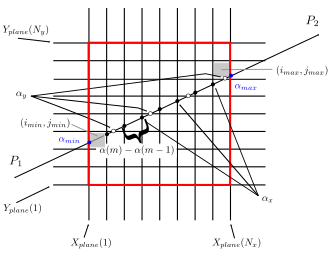
\includegraphics[scale=1.5]{siddon_proj_planes_detail.eps}
\label{fig:siddon_plane_detail}
\caption{a detailed view of the variables in Siddon's algorithm for a 2D plane}
\end{figure}

This process is normally calculated once per ray and would require a simple sorting algorithm that can be provided by either MatLab or C++, and the rays can then be calculated using a standard \textit{for} loop.  However since each ray corresponds to one detector element, and we can utilize the GPU's parallel computation ability to trace all rays simultaneously by assigning each CUDA thread to a single ray.  This can be accomplished by closely following the Siddon's algorithm up until equation \ref{eq:siddon_ijkminmax}.  However since each ray is traced simultaneously, we cannot calculate and sort the set ${\alpha}$ for each ray, instead we have opted to calculate and sort the set ${\alpha}$ on-the-fly where the parametric values ${\alpha_x}$, ${\alpha_y}$, and ${\alpha_z}$ for each ray are calculated on the GPU device memory starting with $\alpha_x(1)$, $\alpha_y(1)$, $\alpha_z(1)$, as  each of the following values ${\alpha_x(i), \alpha_y(j), \alpha_z(k)}$ are calculated for each ray, only the minimum of the three values is used to calculate the ray progression.  As a result, the set ${\alpha}$ is not computed all at once, but rather computed and sorted on-the-fly where only the most current of the two sets, $\alpha(m)$ and 
$\alpha(m-1)$ are stored in device memory.  The number of index, i.e. the number of elements in the set ${\alpha}$ for each ray is given by 
\begin{equation}
n = (i_{max} - i_{min} + 1) + (j_{max} - j_{min}+1) + (k_{max}-k_{min}+1) + 1.
\label{eq:siddon_n}
\end{equation}
Although the number of intersections each ray travels through for each detector element is different, we know when the ray exist the volume.  So we can set a case where once the ray exits the object volume, it will no longer calculate more $\alpha$ values until all rays exists completely through the object volume.  The ray with the maximum number of index $n$, is calculated before the sorting step, along with $\alpha_{min}, \alpha_{max}, i_{min}, i_{max}, j_{min}, j_{max}, k_{min}, and k_{max}$.  While the set of ${\alpha}$ is being sorted on the GPU, the voxel $\left[ i(m), j(m), k(m) \right]$, which corresponds to the intersection created by $m$ and $m-1$ is also calculated each time by
\begin{equation}
\begin{aligned}
i(m) &= 1 + \left[ X_i + \alpha_{mid}(X_2 - X_1) - X_{plane}(1) \right] /d_x, \\
j(m) &= 1 + \left[ Y_i + \alpha_{mid}(Y_2 - Y_1) - Y_{plane}(1) \right] /d_y, \\
k(m) &= 1 + \left[ Z_i + \alpha_{mid}(Z_2 - Z_1) - Z_{plane}(1) \right] /d_z,
\end{aligned}
\label{eq:siddon_voxel}
\end{equation}
where $\alpha_{mid}$ is given by 
\begin{equation}
\alpha_{mid} = \left[ \alpha(m) + \alpha(m-1) \right] /2.
\label{eq:siddon_alphamid}
\end{equation}
The radiological path $d$ may now be written as 

\begin{equation}
\begin{aligned}
d &= \sum\limits_{m = 1}^{m = n} l(m) \rho\left[ i(m), j(m), k(m) \right] \\
  &= d_{12} \; \sum\limits_{m = 1}^{m = n} \left[ \alpha(m) - \alpha(m-1) \right] \rho \left[ i(m), j(m), k(m) \right].
\end{aligned}
\label{eq:siddon_path}
\end{equation}

\begin{sidewaysfigure}
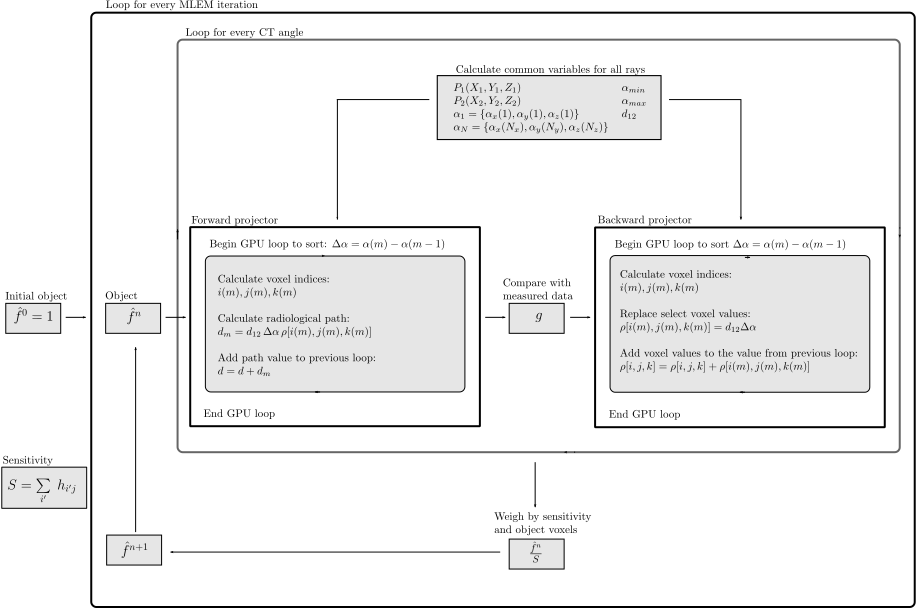
\includegraphics[scale=0.9]{siddon_flowchart.eps}
\caption{A flow chart of Siddon's algorithm implementation on CUDA}
\label{fig:siddon_algorithm_flow_chart}
\end{sidewaysfigure}

Figure \ref{fig:siddon_algorithm_flow_chart} shows a flow chart of how Siddon's algorithm is implemented in CUDA.

\subsection{Forward and backward projector calculation}
The forward projector was implemented following Siddon's algorithm where each x-ray originates from the x-ray source point and travels to the pixel center of each detector element.  The object voxel contribution to the ray was calculated using equation \ref{eq:siddon_path}.  The treatment for the backward projector is very similar to the forward projector, with exception to an added atomicAdd() function in CUDA.  In the forward projection, each voxel index is calculated from the ray intersections, and the voxel value added to each ray is independent of other rays (i.e. Each thread as read-only access to each voxel element and can be added to each ray thread).  However in backward projection, the voxel element needs read and write access since different ray needs access to the same voxel at different times and the voxel thread needs to read the value at that thread and then write to it.  This requires an additional step of using atomicAdd() function.  For further information about atomicAdd() please refer to the CUDA toolkit documentation \cite{Cudatoolkit}.  

\subsection{Sensitivity calculation}

\begin{figure}
\centering
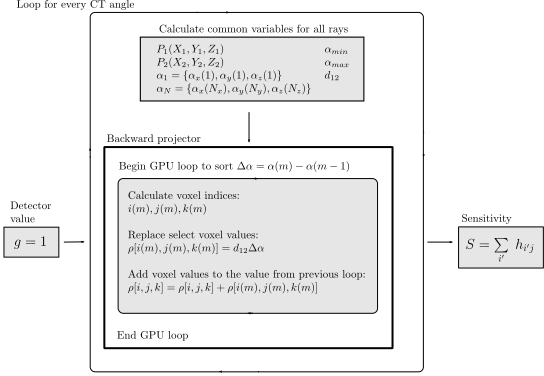
\includegraphics[scale=1]{siddon_flowchart_sensitivity.eps}
\label{fig:sensitivityslices}
\caption{Sensitivity slices using a set of CT parameters, provide a table for the CT parameters}
\end{figure}

The sensitivity used in the MLEM algorithm represents the contribution of all detector values on the object voxel.  This was calculated by first setting all detector values to one, then back filling the object values using the back projector for all scanned angles.  Note that the sensitivity changes depending on the geometry of the CT system, number of object volume, number of detector pixels, and scan routine.  As a result, the sensitivity is always computed in the beginning of each reconstruction event.  However if one were to use a different data set while keeping geometry, object volume, and detector pixels constant, then sensitivity volume does not need to be recalculated and can speed up the reconstruction process.  Figure \ref{fig:sensitivityslices} shows a few slices through the sensitivity volume using a set of CT parameters.
Figure \ref{fig:reconstructedimage} shows the center slice of a reconstructed object after X iterations.

\subsection{Reconstruction results}
The prototype CT system has a XXX field of view, the x-ray magnification can be manually changed along with its optical magnification.  
\comment{
how to show the x-ray magnification, optical magnification as a function of FOV
}
\begin{figure}
\centering
placeholderimage[width=5cm, height=5cm]{reconstructedimage.png}
\label{fig:reconstructedimage}
\caption{reconstructed image slice after X iteration}
\end{figure}
\comment{show reconstruction image for maximum and minimum FOV?}

\subsection{Current algorithm limitations and assumptions}
Here are our assumptions and limitations in the algorithm we've implemented:
\begin{enumerate}
\item Each x-ray originate outside of the object volume, travels completely through the object.  So no ray will ever begin or end inside any voxel.
\item Object volume in each axis are divisible by 4, although it can be modified inside the code.
\item The number of detectors in both the trans-axial and axial directions can only be two to the power of $n$ (i.e. $2^n$ ).
\item Any ray traveling exactly along any voxel plane will not be calculated.
\end{enumerate}


\comment{
in the appendix explain the functions that are included in the algorithm\\
explain how to checkout the repository (nvm)\\
how to use the parameter file \\
what are the outputs of each function (recon, forward, backward)
}


\section{Filtered Back-Projection (FBP) }


